\documentclass[../uilmath.tex]{subfiles}
\graphicspath{{\subfix{../figures/}}}
\begin{document}
\chapter{Calculus}
\section*{Problems}
\begin{enumerate}[label=\bfseries\arabic*.]
    \item %% Problem 1
    Find the area of the shaded region (nearest square unit)
    \begin{center}
        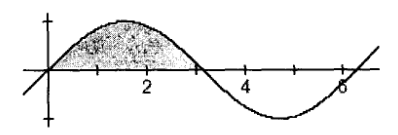
\includegraphics[width=0.3\textwidth]{2006SAC20.PNG}
    \end{center}

    \item %% Problem 2
    Which of the following sequences is divergent?

    $\textbf{(A)} \left\{\frac{2n+1}{3n-2}\right\}\qquad \textbf{(B)}\left\{\frac{-1^n}{n^2+n}\right\}\qquad \textbf{(C)}\left\{\frac{(-1)^n(n+1)}{n+2}\right\}\qquad \textbf{(D)}\left\{\frac{4n^2-n^3}{10+2n^3}\right\}\qquad \textbf{(E)}\left\{\frac{6n^2+3n-1}{n^2+8n+16}\right\}$

    \item %% Problem 3
    If $f'(x)=6x^2-4x+1$ and $f(1)=0$, find $f(-1)$.

    \item %% Problem 4
    $f(x)=2x^3-6x+1$ has an inflection point at:
    
    \item %% Problem 5
    Find the area (in square units) of the region bounded by $x=\frac{y^2+2}{2}$ and $x=y+5$.

    \item %% Problem 6
    The graph of $f'(x)$ is shown below. If $f(1)=2\frac{1}{3}$, then $f(2)=\blank$.
    \begin{center}
        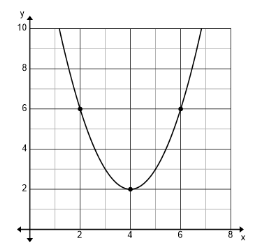
\includegraphics[width=0.3\textwidth]{2021SAC9.PNG}
    \end{center}
    
    \item %% Problem 7
    \begin{center}
        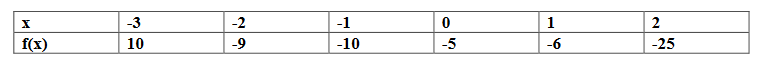
\includegraphics[width=0.3\textwidth]{2021SAC26.PNG}
    \end{center}

    The point of inflection for the graph of $f(x)$ has coordinates $(a,b)$. $a+b=\blank$. (nearest tenth)


    The following graph is used for problems 8 and 9.
    \begin{center}
        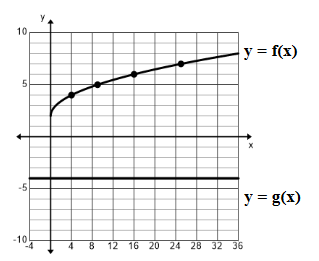
\includegraphics[width=0.3\textwidth]{2021SAC42.PNG}
    \end{center}
    \item %% Problem 8
    Find the area between the curves $y=f(x)$ and $y=g(x)$ shown on the right over the interval $[4,24]$. (nearest whole number)

    \item %% Problem 9
    Find the volume of the solid generated by revolving the region bounded by $y=f(x)$, the $x$-axis, the line $x=4$ and 
    the line $x=24$ about the line $y=g(x)$. (nearest whole number)

    \item %% Problem 10
    Find the area of one petal of the rose curve $r=6\cos(2\theta)$. (nearest tenth)

    \item %% Problem 11
    Find the interval of convergence for the power series $\sum_{n=1}^\infty \frac{(-1)^{n+1}x^n}{4^n}$.

    \item %% Problem 12
    Find the value of $c$ in the open interval $(-8,2)$ that satisfies the mean value theorem for the function 
    $f(x)=\sqrt{6-x}$. (nearest hundredth)

    \item %% Problem 13
    If you were going to evlauate $\int \frac{\cos x}{\sin^3 x}\mathrm{d}x$ using $u$-substitution, the best choice for $u$ is \blank.

    \item %% Problem 14
    If $f(x)=x^2-8x+9$, then $\frac{f(x+h)-f(x)}{h}=\blank$.

    \item %% Problem 15
    Find the area bounded by thw two curves shown below. (nearest tenth)
    \begin{center}
        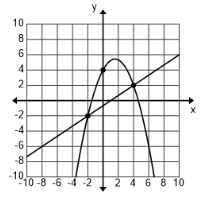
\includegraphics[width=0.3\textwidth]{2022SAC40.PNG}
    \end{center}

    \item %% Problem 16
    Consider the function $f(x)=\frac{1}{2}\cos(2x)+\frac{3}{2}\sin(x)$. Find the slope of the line tangent to 
    the graph of $y=f(x)$ when $x=\pi$. (nearest tenth)

    \item %% Problem 17
    A balloon is rising straight up from a point on the ground 150 feet from a curious mouse. If the balloon is rising at a 
    rate 8 ft/s, what is the rate of change of the angle of elevation of the balloon from the mouse when the balloon is 200 ft above the groud. (nearest hundredth)

    \item %% Problem 18
    A rectangular solid with a square base has a total surface area of 330 in$^2$. Find the maximum volume possible for such a solid. (nearest tenth)


    Use the following graph for questions 19 and 20.
    \begin{center}
        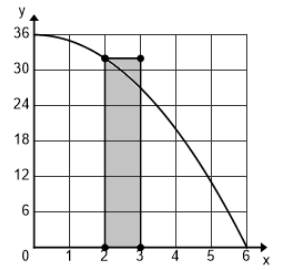
\includegraphics[width=0.3\textwidth]{2022SAC45.PNG}
    \end{center}
    \item %% Problem 19
    Find an approximation of the area bounded by the graph of $f(x)=36-x^2$ and the $x$-axis between $x=1$ and $x=5$. 
    Use four rectangles of equal width and find the height of each rectangle using the left endpoint of the interval. One of the rectangles is shown above.

    \item %% Problem 20
    Find the exact area of the region bounded by the graph of $f(x)=36-x^2$ and the $x$-axis between $x=1$ and $x=5$. (nearest tenth)

    \item %% Problem 21
    Find the derivative of $F(x)$ if $F(x)=\int_0^{4x}\sin(t)\mathrm{d}t$.

    \item %% Problem 22
    When evaluating $\int x^2\cos(x)\mathrm{d}x$ using a $u$-substitution, the best choice for $u$ is $\blank$.

    \item %% Problem 23
    Let $f(x)=\sin(x)$ and let $P_5(x)$ be the fifth Maclaurin polynomial for $f(x)=\sin(x)$. Find the value of 
    $\left|P_5\left(\frac{\pi}{6}\right)-f\left(\frac{\pi}{6}\right)\right|$. (nearest ten-millionth)

    \item %% Problem 24
    Find the length of the arc from $\theta=\frac{\pi}{6}$ to $\theta=\frac{\pi}{3}$ for the polar curve $r=4-4\cos(\theta)$. (nearest tenth)

    \item %% Problem 25
    
\end{enumerate}

\section*{Solutions}
\begin{enumerate}[label=\bfseries\arabic*.]
    \item %% Problem 1
    2

    \item %% Problem 2
    C 

    \item %% Problem 3
    -6

    \item %% Problem 4
    $(0,1)$

    \item %% Problem 5
    18 

    \item %% Problem 6
    $10\frac{2}{3}$

    \item %% Problem 7
    -8.0

    \item %% Problem 8
    193

    \item %% Problem 9
    4890 

    \item %% Problem 10
    14.1

    \item %% Problem 11
    $(-4,4)$

    \item %% Problem 12
    -2.24

    \item %% Problem 13
    $\sin x$

    \item %% Problem 14
    $2x+h-8, h\neq 0$

    \item %% Problem 15
    21.0

    \item %% Problem 16
    -1.5

    \item %% Problem 17
    0.02 rad/s 

    \item %% Problem 18
    407.9 in$^3$

    \item %% Problem 19
    114

    \item %% Problem 20
    102.7

    \item %% Problem 21
    $4\sin(4x)$

    \item %% Problem 22
    $x^2$

    \item %% Problem 23
    0.0000021

    \item %% Problem 24
    1.6

    \item %% Problem 25
    
\end{enumerate}


\end{document}